<<<<<<< HEAD
\chapter{Results}
\section{Simulation of Capacitance values}
\subsection{Comparision of Capacitance in the simulation with a sphere geometry}
The simulation of the capacitance for the cylindric geometry as a function of different distances with COMSOL leads to the following figure.The simulation of two spheres as well as the approximation formula result in a general shift which is due to the fact that it is a three electrode arrangement as the wall of the low-voltage introduces a new capacitance between the upper electrode and the wall which is not affected by the distance variation. This results in a reduction of the capacitance compared to the two spheres geometry. Thus, the simulated values for the low voltage test cell seem reasonable if one compares them to the results of the capacitance between two spheres. \newline 


\begin{figure}[]
	\centering
	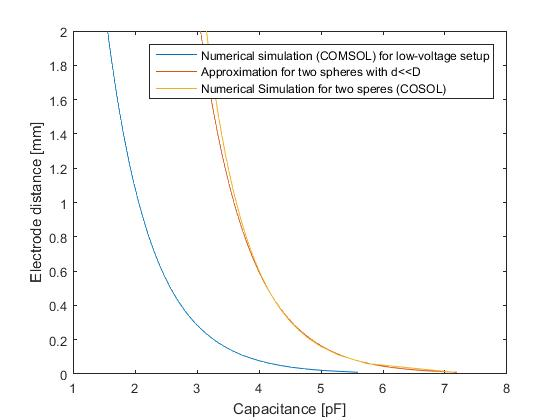
\includegraphics[scale=0.3]{figures/Comparison_Low_voltage_Two_spheres}		
	\caption[Kurze Abbildungsbeschreibung]{Dependency of the electrode distance on the capacitance for the low voltage setup and two spheres $\epsilon = 3.5$ } 
	\label{fig.waveforms}
\end{figure}

\section{Complex effective permittivity}
\subsection{}
=======
\chapter{Results}
\section{Simulation of Capacitance values}
\subsection{Comparision of Capacitance in the simulation with a sphere geometry}
The simulation of the capacitance for the cylindric geometry as a function of different distances with COMSOL leads to the following figure.The simulation of two spheres as well as the approximation formula result in a general shift which is due to the fact that it is a three electrode arrangement as the wall of the low-voltage introduces a new capacitance between the upper electrode and the wall which is not affected by the distance variation. This results in a reduction of the capacitance compared to the two spheres geometry. Thus, the simulated values for the low voltage test cell seem reasonable if one compares them to the results of the capacitance between two spheres. \newline 


\begin{figure}[htbp]
	\centering
	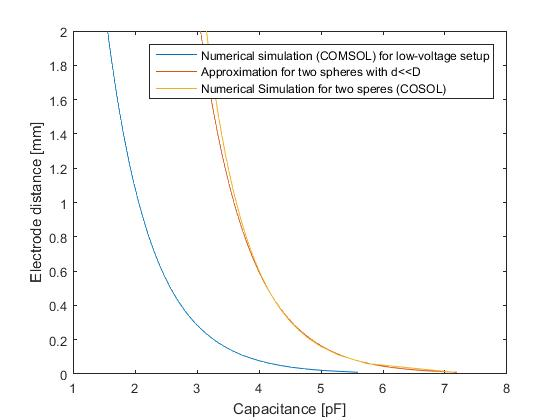
\includegraphics[scale=0.3]{figures/Comparison_Low_voltage_Two_spheres}		
giit 	\caption[Kurze Abbildungsbeschreibung]{Dependency of the electrode distance on the capacitance for the low voltage setup and two spheres (\epsilon = 3.5) } %\ref{sec.analysecurrent}
	\label{fig.waveforms}
\end{figure}

\section{Complex effective permittivity}
\subsection{}

\section{Performance of integrator}

\section{Dielectric Spectroscopy}

\begin{figure}[htbp]
\end{figure}
>>>>>>> origin/master
